% !TEX root = ../main.tex

\section{Experimental Results}
\label{sec:orgc23a664}

We show results on four different datasets, moviePosters, cancerHallmarks, chemicalExposure and Arxiv2020.
Interestingly, tencentLoss and focalLoss, which are specifically tailored for sparse data, do not perform well here. Note that macroSoftF1 can be particularly performent without requiring hyperparameter tuning. Across Tables \ref{tab:chemicalExposure, tab:moviePosters, tab:arxiv2020, tab:cancerHallmarks} we see that the smooth sigmoidF1 outperforms other existing losses. Although only the metrics@0.5 are shown, where 0.5 is the dichotomization threshold, the ablation study and our open sourced code further illustrates the consistent good performance of sigmoidF1 versus other losses.


For the two medical datasets cancerHallmarks and chemicalExposure, information is a lot more sparse, we thus set the evaluation metrics threshold at 0.05 and train for 500 epochs until reaching convergence. 

\subsection{Ablation Study - Arxiv2020}

We performed an analysis of sensitivity to different amount of labels. For this, the irrelevance threshold (see definition in Section \ref{sec:orgb44ba25}) $t$ was set to the values 0, 10, 100 and 1000. This time, results are shown with dichotomization thresholds of 0.1 to 0.9. \todo{see if keep it}

\todo{sensitivity to hyperparametertuning plot}

\begin{figure}[htbp]
\centering
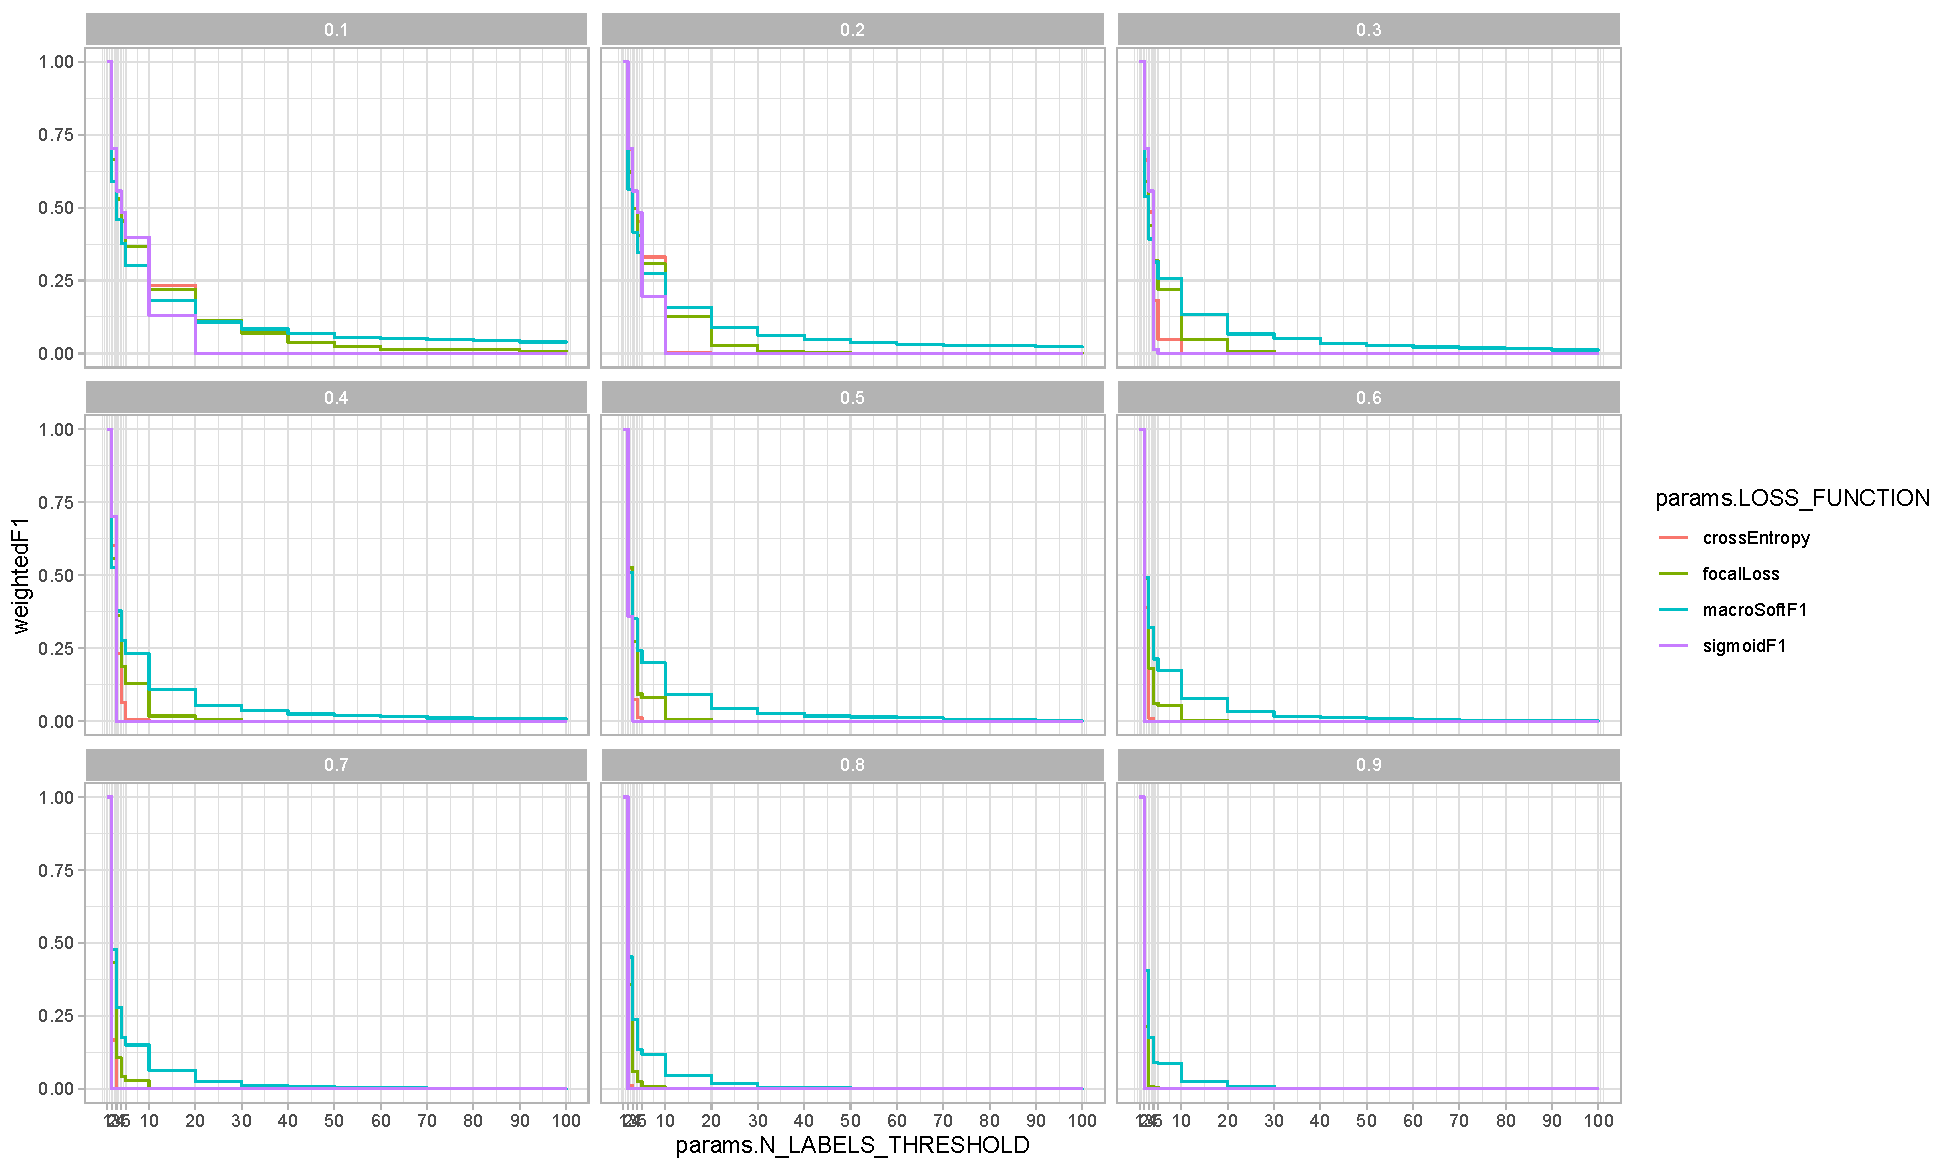
\includegraphics[width=.9\linewidth]{./images/ablation.pdf}
\caption{\label{fig:ablation}
Sigmoid function with different values for $\beta$ (steepness) \& $\eta$ (offset)}
\end{figure}


\todo{change to percentage}

\begin{table}
  \caption{Movie posters (CNN). \mdr{Explain what we see.}}
  \label{tab:moviePosters}
\centering
\begin{tabular}{l ccccc}
\toprule 
Loss  & \rotatebox{90}{macroF1 @ 0.5} & \rotatebox{90}{microF1 @ 0.5} & \rotatebox{90}{weightedF1 @ 0.5} & \rotatebox{90}{Precision @ 0.5} & \rotatebox{90}{Recall @ 0.5}\\ 
\midrule
$\mathcal{L}_{\text {CE}}$ & 0.051 & 0.186 & 0.149 & 0.090 & 0.042 \\ 
$\mathcal{L}_{\text {FL}}$ & 0.055 & 0.192 & 0.154 & 0.115 & – \\
% $\mathcal{L}_{\text {CE+N}}$ & 0 & 0 & 0 & 0 & 0 \\
$\mathcal{L}_{\text {macroSoftF1}}$ & 0.136 & 0.207 & 0.243 & \textbf{0.105} & 0.190 \\
$\mathcal{L}_{\text {sigmoidF1}}$ & \textbf{0.158} & \textbf{0.224} & \textbf{0.300} & 0.104 & \textbf{0.557} \\ % run aa424792a57e4208ad1805cd6e63f8e6
\bottomrule
\end{tabular}
\end{table}


\begin{table}
  \caption{Arxiv (distillBERT 2020), frozen pretrained weights 100 epochs, min-label-thresh: 1000}
  \label{tab:arxiv2020}  
\centering
\begin{tabular}{l ccccc}
\toprule
Loss  & \rotatebox{90}{macroF @ 0.5} & \rotatebox{90}{microF1 @ 0.5} & \rotatebox{90}{weightedF1 @ 0.5} & \rotatebox{90}{Precision @ 0.5} & \rotatebox{90}{Recall @ 0.5}\\ 
\midrule
$\mathcal{L}_{\text {CE}}$ & 0.093 & 0.106 & 0.106 & 0.096 & – \\ % Run 71ef078f975649d5b3d897e504bc638b
$\mathcal{L}_{\text {FL}}$ & 0.008 & 0.011 & 0.009 & 0.054 & 0.954 \\
% $\mathcal{L}_{\text {CE+N}}$ & 0 & 0 & 0 & 0 & 0 \\
$\mathcal{L}_{\text {macroSoftF1}}$ & 0.077 & 0.088 & 0.087 & 0.100 & – \\ % run 405a6e6851e84a89a82313251a7a36e8 (18-19 jan)
$\mathcal{L}_{\text {sigmoidF1}}$ & \textbf{0.093} & \textbf{0.106} & \textbf{0.106} & \textbf{0.096} & \textbf{–} \\ % run bd478ca55eb64cc78d9ad0f25accce35 (18-19 jan)
\bottomrule
\end{tabular}
\end{table}

\begin{table}
  \caption{Cancer Hallmarks}
  \label{tab:cancerHallmarks}
\centering
\begin{tabular}{l ccccc}
\toprule 
Loss  & \rotatebox{90}{macroF1 @ 0.05} & \rotatebox{90}{microF1 @ 0.05} & \rotatebox{90}{weightedF1 @ 0.05} & \rotatebox{90}{Precision @ 0.05} & \rotatebox{90}{Recall @ 0.05}\\ 
\midrule
$\mathcal{L}_{\text {CE}}$ & 0.0 & 0.0 & 0.0 & 0.0 & 0.0 \\ 
$\mathcal{L}_{\text {FL}}$ & 0.044 & 0.190 & 0.108 & 0.071 & 0.055 \\
% $\mathcal{L}_{\text {CE+N}}$ & 0 & 0 & 0 & 0 & 0 \\
$\mathcal{L}_{\text {macroSoftF1}}$ & 0.098 & 0.176 & 0.170 & 0.089 & 0.131 \\
$\mathcal{L}_{\text {sigmoidF1}}$ & \textbf{0.095} & \textbf{0.313} & \textbf{0.202} & \textbf{0.059} & \textbf{0.264} \\ % run e145056949424b02bfc83cc57af38374
\bottomrule
\end{tabular}
\end{table}


\begin{table}
  \caption{Chemical Exposure}
  \label{tab:chemicalExposure}
\centering
\begin{tabular}{l ccccc}
\toprule
Loss  & \rotatebox{90}{macroF1 @ 0.05} & \rotatebox{90}{microF1 @ 0.05} & \rotatebox{90}{weightedF1 @ 0.05} & \rotatebox{90}{Precision @ 0.05} & \rotatebox{90}{Recall @ 0.05}\\ 
\midrule
$\mathcal{L}_{\text {CE}}$ & 0.012 & 0.058 & 0.051 & 0.047 & 0.007 \\ % Run 71ef078f975649d5b3d897e504bc638b
$\mathcal{L}_{\text {FL}}$ & 0.0934 & 0.348 & 0.268 & 0.130 & 0.091 \\
$\mathcal{L}_{\text {macroSoftF1}}$ & 0.133 & 0.194 & 0.218 & 0.155 & 0.138 \\ % run 405a6e6851e84a89a82313251a7a36e8 (18-19 jan)
$\mathcal{L}_{\text {sigmoidF1}}$ & \textbf{0.113} & \textbf{0.432} & \textbf{0.319} & \textbf{0.091} & \textbf{0.188} \\ % run a30825efe9c94a24bc46a9c71a5f8646 E: 0.5 S: 0.6
\bottomrule
\end{tabular}
\end{table}


%%% Local Variables:
%%% mode: latex
%%% TeX-master: "../main"
%%% End:
